\documentclass[../main.tex]{subfiles}

\makeatletter
\@ifundefined{fromRoot}{%
  \newcommand{\fromRoot}[1]{../#1}
  
  \usepackage{xr}
  \externaldocument{../main}
}{}

\def\input@path{{\subfix{../}}}
%or: \def\input@path{{/path/to/folder/}{/path/to/other/folder/}}
\makeatother

\graphicspath{{\subfix{../}}}

\hypersetup{
    pdfauthor   = {Camille MONIÈRE},
    pdftitle    = {Th\`{e}se (Présentation: contexte)},
    pdfsubject  = {Th\`{e}se (Présentation: contexte)},
%    pdfkeywords = {mots-cl\'{e}s},
}

\begin{document}

\section{Introduction}

\subsection{Contexte}

\begin{frame}{Télécommunications numériques sans-fil}
  \begin{columns}
    \begin{column}{.4\linewidth}
      \begin{center}
        \placeholder{width=.85\linewidth, height=.6\textheight}
        \captionof{figure}{Illustration : une antenne, deux devices.}
      \end{center}
    \end{column}
    \begin{column}{.55\linewidth}
      \small
      \begin{overlayarea}{\linewidth}{.6\textheight}
        \begin{ctrlitemize}{1em}
          \item Plus fiables et résilients que leurs pendants analogiques.
          \item<2-> Champ regroupant :
          \begin{ctrlitemize}{1ex}
            \scriptsize
            \item<2-> les réseaux cellulaires \\\hspace{1em} \textit{3G, 4G/LTE, 5G},
            \item<3-> les réseaux en champs proches \\\hspace{1em} \textit{ZigBee, NFC, Bluetooth},
            \only<4>{\item et les réseaux longues portées basses puissances \acrshortpl{lpwan} \\\hspace{1em} \textit{LoRa/LoRaWAN, SigFox, NB-IoT}.}
            \only<5->{\item et \textbf{\textcolor{red}{les réseaux longues portées basses puissances \acrshortpl{lpwan}}} \\\hspace{1em} \textit{LoRa/LoRaWAN, SigFox, NB-IoT}.}
          \end{ctrlitemize}
        \end{ctrlitemize}
      \end{overlayarea}
    \end{column}
  \end{columns}
\end{frame}

\begin{frame}{\acrfullpl{lpwan}}
  \small
  \begin{overlayarea}{\linewidth}{.1\textheight}
    \only<1>{
      Fort développement de l'\acrfull{iot} \textit{[internet des objets]} durant la dernière décennie
      \textcolor{red}{$\Rightarrow$} développement des \acrshortpl{lpwan}\cite{IEEEStandardLPWAN}.
    }
    \only<2>{
      Le \acrshortpl{lpwan} ont connu un fort développement durant la dernière décennie, de nombreux standards ont vu le jour\cite{goursaudDedicatedNetworksIoT2015, sinhaSurveyLPWATechnology2017}.%
    }
  \end{overlayarea}

  \begin{overlayarea}{\linewidth}{.65\textheight}
    \only<1>{
      \begin{columns}
        \begin{column}{.4\linewidth}
          \scriptsize
          Caractéristiques des \acrshortpl{lpwan} :
          \begin{ctrlitemize}{4pt}
            \item portées longues,
            \item coûts faibles,
            \item consommations énergétiques réduites.
          \end{ctrlitemize}
          $\Rightarrow$ Permettre le déploiement massif de d'objets connectés alimentés par batterie.\\
          $\Rightarrow$ Requiert des débits plus faibles, que les réseaux cellulaires notamment.
        \end{column}
        \begin{column}{.5\linewidth} \centering
          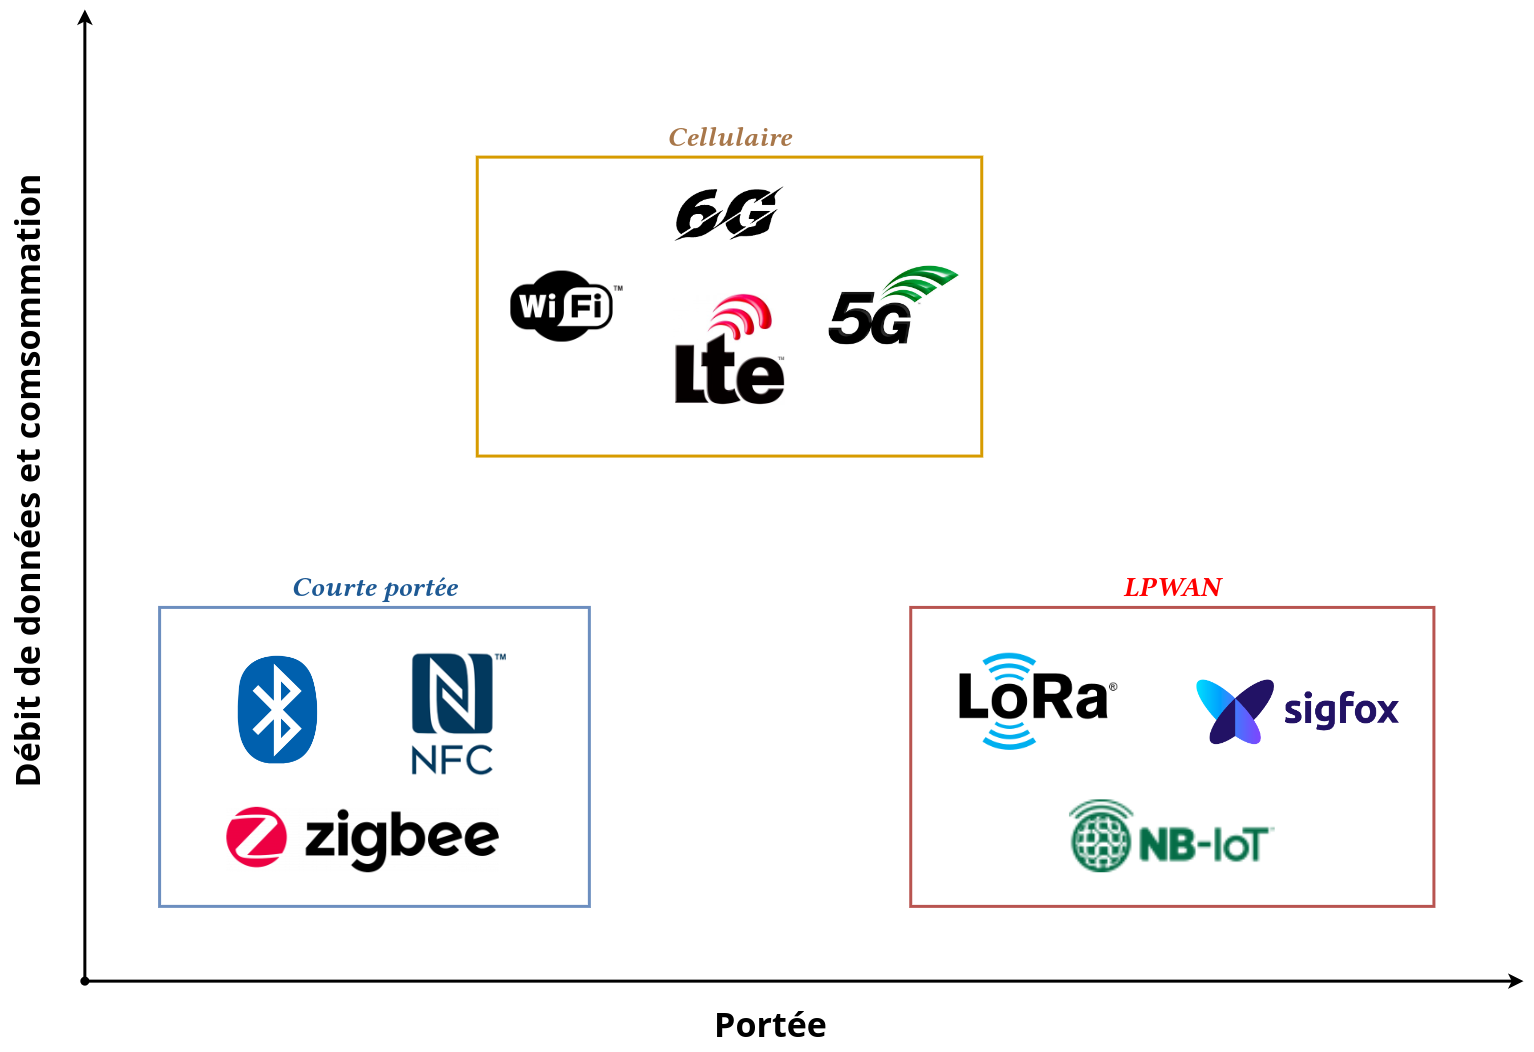
\includegraphics[width=\linewidth]{figures/drawiopdf/lpwan_and_co}
          \captionof{figure}{Aperçu des caractéristiques de trois technologies utilisées dans les \acrshortpl{lpwan}, SigFox, LoRa et NB-IoT.}
        \end{column}
      \end{columns}
    }
    \only<2>{
      \begin{center}
        \ra{1.3}
        % \begin{noindent}
          \scriptsize
          \begin{tabular}[t]{@{}r@{\phantom{XXX}}r@{\phantom{XX}}r@{\phantom{XX}}r@{}}
            \toprule
                                   & \textbf{SigFox}   & \textbf{LoRa}     & \textbf{NB-IoT}     \\ \midrule
            \textbf{Modulation}    & \acrshort{bpsk}   & \acrshort{css}    & \acrshort{qpsk}     \\ 
            \textbf{Fréquence centrale}
                                   & $868$ MHz         & $868$ MHz         & bandes LTE          \\
            \textbf{Largeur de bande}
                                   & $0.1$ kHz         & $125$/$250$ kHz   & $200$ kHz           \\
            \textbf{Débit max de données} 
                                   & $0.1$ kb/s        & $50$ kb/s         & $200$ kb/s          \\
            \textbf{Taille max de la charge utile}
                                   & $96$ bits         & $1944$ bits       & $12.8$ kilobits     \\
            \textbf{Portée urbaine}
                                   & $10$ km           & $5$ km            & $1$ km              \\
            \textbf{Portée rurale} & $40$ km           & $20$ km           & $10$ km             \\
            \textbf{Résilience aux interférences}
                                   & très grande       & très grande       & basse               \\
            \textbf{Code(s) correcteur(s) d'erreur}
                                   & aucun             & codes de Hamming  & codes conventionnel \\
            \bottomrule
          \end{tabular}
          % \end{noindent}
        \captionof{table}{Aperçu des caractéristiques de trois technologies utilisées dans les \acrshortpl{lpwan}, SigFox, LoRa et NB-IoT.}
        \ra{1}
      \end{center}
    }
  \end{overlayarea}
  \only<1>{\blfootnotetext{\textcite{IEEEStandardLPWAN}}}
  \only<2>{
    \blfootnotetext{\textcite{goursaudDedicatedNetworksIoT2015, sinhaSurveyLPWATechnology2017}}
  }
\end{frame}


\begin{frame}{Problème des préambules}
  % \begin{overlayarea}{\linewidth}{.05\textheight}
  % \end{overlayarea}
  \begin{columns}
    \begin{column}{.25\linewidth}
      \begin{overlayarea}{\linewidth}{.45\textheight}
        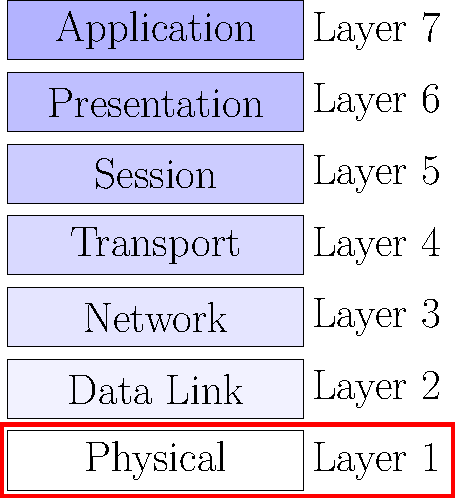
\includegraphics[width=\linewidth]{figures/tikzpicture/osi_layers_stdl}
      \end{overlayarea}
    \end{column}
    \begin{column}{.02\linewidth}
    \end{column}
    \begin{column}{.69\linewidth}
      \begin{overlayarea}{\linewidth}{.45\textheight}
        \only<1,2>{
          \includegraphics[width=\linewidth]{figures/tikzpicture/joint_frame_tikz_bare.pdf}
        }
        \only<3>{
          \includegraphics[width=\linewidth]{figures/tikzpicture/joint_frame_tikz.pdf}
        }
      \end{overlayarea}
    \end{column}
  \end{columns}

  \begin{overlayarea}{\linewidth}{.4\textheight}
    \only<1>{
      \includegraphics[width=\linewidth]{figures/tikzpicture/joint_frame_tikz_leg.pdf}
    }
    \only<2->{ \centering
    \includegraphics[width=\linewidth]{figures/tikzpicture/joint_frame_tikz_leg-2.pdf}\\
    {\tiny \fullcite{polyanskiyAsynchronousCommunicationExact2013}}
    }
  \end{overlayarea}
\end{frame}


\subsection[Le projet \acrshort{qcsp}]{Le projet \acrfull{qcsp}}

\begin{frame}{\subsecname}{}
  \begin{center}
    
\includegraphics[width=0.6\linewidth]{figures/logos-thesis/partners-logos.png}
  \end{center}
\end{frame}

\begin{frame}{Principes de \acrshort{qcsp}}
  \textbf{TODO, le spatial, le ccsk et le nbldpc}
\end{frame}

\begin{frame}{\acrfull{ccsk}}
  \textbf{TODO, animation comment on module et comment on démodule}
\end{frame}

\begin{frame}{\acrfull{ldpc}}
  \textbf{TODO, TRES SUCCINCT, vitye fait trois VN et un CN, pour completion}
\end{frame}


\end{document}
